\titlepageframe % Specific command 

\begin{tframe}{Motivación}
	\begin{block}<1->{Serie temporal. Definición}
		Secuencia de datos medidos en determinados momentos y ordenados cronológicamente, pudiendo estar estos datos espaciados a intervalos iguales o desiguales.
	\end{block}
	\begin{itemize}
		\item Tipo de dato de enorme importancia en múltiples campos.
		\item Diversos tipos de métodos para analizarlas y predecir valores futuros.
		\item<+-> A falta de una biblioteca que englobe estos métodos y plataforma desde la que aplicarlos...
		\item<+-| alert@+> TimeSeriesAnalysis
	\end{itemize}
\end{tframe}

\begin{tframe}{Objetivos}
	\begin{block}<1->{Sistema clasificador}
		\begin{itemize}
			\item Usando una serie temporal almacenada
			\item A partir del conocimiento obtenido de todas las series temporales almacenadas
			\item Calcula la complejidad de la serie temporal
			\item La clasifica comparando su complejidad con la de las demás
		\end{itemize}
	\end{block}
\end{tframe}

\begin{tframe}{Objetivos (II)}
	\begin{block}<1->{Biblioteca de métodos de análisis}
		\begin{itemize}
			\item Incluye métodos de análisis (medidas de complejidad), predicción y transformación de series temporales
			\item Además se han añadido métodos para clustering
			\item Y funciones básicas para trabajar con datos y series temporales
			\item El sistema clasificador hace uso de esta biblioteca
		\end{itemize}
	\end{block}
	\begin{block}<2->{Plataforma web}
		\begin{itemize}
			\item Aplicación web de fácil uso para el usuario
			\item Funciona junto a la biblioteca y la base de datos de series temporales
		\end{itemize}
	\end{block}
\end{tframe}

\begin{tframe}{Metodología}
	\begin{block}<1->{SCRUM}
		Metodología de desarrollo ágil caracterizada por tener una estrategia de desarrollo incremental, ejecución completa del producto por 			intervalos, equipos de desarrollo auto organizados y solapamiento de las diferentes fases del desarrollo.
	\end{block}
	\begin{block}<2->{MVC}
		Arquitectura de software que divide el desarrollo de un sistema en tres módulos o partes principales, separando la interfaz de usuario (vista) de la lógica (controlador) y los datos (modelo).
	\end{block}
\end{tframe}

\begin{tframe}{Herramientas}
	\begin{itemize}
		\item Git
		\item Docker
		\item RStudio
		\item PhpStorm
		\item PyCharm
		\item Youtrack
		\item Teamcity
		\item Visual Paradigm
		\item InfluxDB
		\item Apache
		\item PhpMyAdmin
	\end{itemize}	
\end{tframe}

\begin{tframe}{Herramientas (II)}
	\begin{itemize}
		\item Paquetes R: R6, parallel, Rcpp, bigmemory, testthat, ...
		\item Paquetes PHP (Composer): influxdb-php, slim, phpunit, ...
		\item Paquetes NPM: angular, bootstrap, highcharts, karma, ...
	\end{itemize}	
\end{tframe}

\begin{tframe}{Medidas de complejidad}
	\begin{block}<1->{Definición}
		Cálculo que se aplica sobre un conjunto de datos, en este caso series temporales, y devuelve como resultado el grado de dificultad de los datos de esta para analizarlos.
	\end{block}
	\begin{itemize}
		\item Los resultados de complejidad son usados para la clasificación
		\item Las medidas de complejidad que han sido implementadas: Kolmogorov, Lempel-Ziv, Aproximation-Entropy, Sample Entropy, Permutation Entropy, Shannon Entropy, ChaoShen Entropy, Dirichlet Entropy, MillerMadow Entropy, Shrink Entropy.
	\end{itemize}
\end{tframe}

\begin{tframe}{Análisis del conjunto de series temporales}
	\begin{itemize}
		\item Dependiente de los métodos implementados en la biblioteca
		\item El resultado obtenido en este análisis es un sistema clasificador
		\item Los últimos resultados se ejecutaron sobre un conjunto de 60000 series temporales
	\end{itemize}
	\begin{block}<1->{Medidas de complejidad}
		\begin{itemize}
			\item<+-| alert@+> Sobre todas las series temporales se aplican todas las medidas de complejidad
			\item<+-| alert@+> Esta matriz de 60000x10 se almacena en la base de datos, cada serie temporal con sus resultados de complejidad
			\item<+-| alert@+> Se almacenan para una ejecución de los experimentos más rápida, las medidas de complejidad de cada serie temporal solo son calculadas una vez.
		\end{itemize}
	\end{block}
\end{tframe}

\begin{tframe}{Análisis del conjunto de series temporales (II)}
	\begin{block}<1->{Clustering}
		\begin{itemize}
			\item<+-| alert@+> A la matriz de medidas de complejidad se le aplica Clustering
			\item<+-| alert@+> Los métodos de clustering usados han sido: KMeans y CMeans
			\item<+-| alert@+> Son métodos no-jerárquicos
			\item<+-| alert@+> Como método para el cálculo de centros se han implementado el método de Chiu
			\item<+-| alert@+> Para 60000 series temporales se obtuvieron 129 centros
			\item<+-| alert@+> Se seleccionó el método KMeans, ya que es el que generaba mejores resultados, en las comparaciones del experimento
			\item<+-| alert@+> Al igual que con las medidas de complejidad los resultados de clustering se almacenan en la base de datos
		\end{itemize}
	\end{block}
\end{tframe}

\begin{tframe}{Análisis del conjunto de series temporales (III)}
	\begin{block}<1->{Clasificación}
		\begin{itemize}
			\item<+-| alert@+> Sobre cada grupo obtenido se aplican todos los métodos de predicción a cada serie temporal, del grupo. Se selecciona el método con menor error.
			\item<+-| alert@+> El método de predicción para cada centro se guarda en base de datos.
			\item<+-| alert@+> Para clasificar una nueva serie temporal se calculan sus medidas de complejidad y con una función de distancia a todos los centros se selecciona el de menor distancia 
			\item<+-| alert@+> Se devuelve el grupo y el método de predicción que se le asignó.
		\end{itemize}
	\end{block}
\end{tframe}

\begin{tframe}{Análisis del conjunto de series temporales (IV)}
\begin{block}<1->{Sistema Clasificador: Características}
	\begin{itemize}
		\item<+-| alert@+> Usa la API para obtener las series temporales y, obtener y almacenar los resultados
		\item<+-| alert@+> Se han desarrollado scripts en R específicos para el análisis
		\item<+-| alert@+> En algunas clases R ha sido necesario implementarlas en C++ debido a los altos requisitos de computación (Ejemplo: Cáculo de centros Chiu)
		\item<+-| alert@+> Se han desarrollado varios paquetes R
		\item<+-| alert@+> Los paquetes R más importantes para el sistema clasificador son:
		\begin{itemize}
			\item<+-| alert@+> Clustering
			\item<+-| alert@+> TimeSeriesDatabase
			\item<+-| alert@+> TimeSeriesComplexity
		\end{itemize}
	\end{itemize}
\end{block}
\end{tframe}

\begin{tframe}{Sistema: Despliegue en Cloud}
	\begin{itemize}
		\item<+-| alert@+> Con el fin de conseguir una aplicación distribuida se ha usado el software Docker
		\item<+-| alert@+> Se ha desarrollado un script en Python para gestionar todos los contenedores Docker (DockersProject)
		\item<+-> Los contenedores usados han sido:
		\begin{itemize}
			\item TimeSeriesAnalysisWebApp
			\item TimeSeriesAnalysisAPI
			\item MySQL
			\item PhpMyAdmin
			\item InfluxDB
			\item TeamCity
			\item YouTrack
			\item TeamCity Agent 1-3
		\end{itemize}
	\end{itemize}
\end{tframe}

\begin{tframe}{Sistema: Despliegue en Cloud (II)}
	\begin{center}
		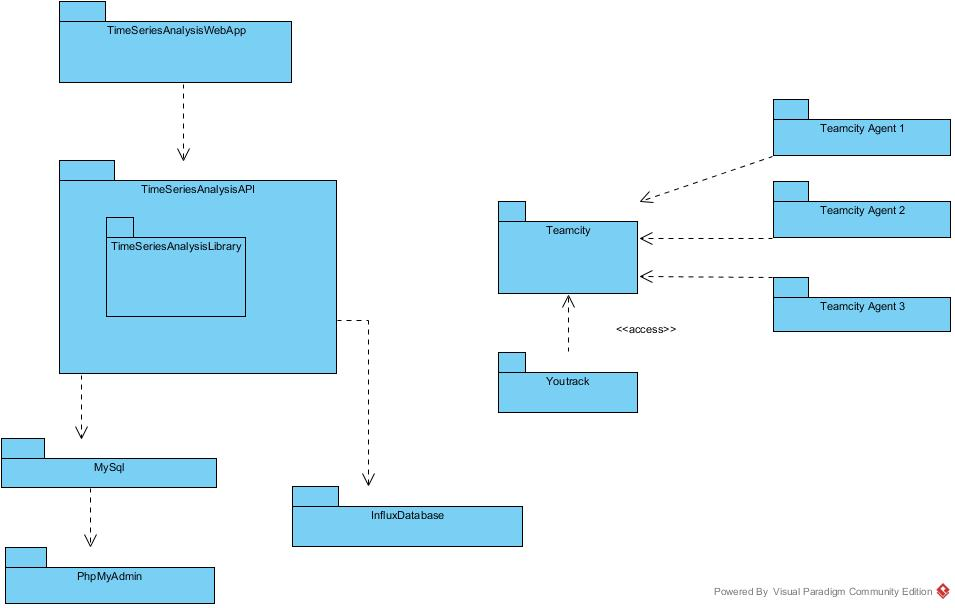
\includegraphics[scale=0.28]{images/DockerContainers}
	\end{center}
\end{tframe}

\begin{tframe}{Conclusiones}
	El proyecto desarrollado se compone de tres módulos principales:
	\begin{itemize}
		\item<+-| alert@+> Biblioteca de análisis (TimeSeriesAnalysisLibrary)
		\item<+-| alert@+> API (TimeSeriesAnalysisAPI)
		\item<+-| alert@+> Plataforma web (TimeSeriesAnalysisWebApp)
	\end{itemize}
\end{tframe}

\begin{tframe}{Conclusiones (I)}
	\begin{block}<1->{TimeSeriesAnalysisLibrary}
		Módulo formado por varios paquetes R que incluyen todos los métodos de análisis utilizados y la funcionalidad que ha sido necesaria desarrollar para trabajar con series temporales.
	\end{block}
	\begin{block}<2->{TimeSeriesAnalysisAPI}
		Este módulo contiene toda la funcionalidad necesaria para una API, escrita en PHP.
	\end{block}
	\begin{block}<3->{TimeSeriesAnalysisWebApp}
		Plataforma web escrita en javascript usando el framework Angular.
	\end{block}
\end{tframe}

\begin{tframe}{Conclusiones (II)}
	\begin{center}
		\highlightbf{¿Preguntas?}
	\end{center}
\end{tframe}